\subsection{Caso em que apenas $K_p$ � desconhecido}

\begin{align*}
P(s) &= \begin{bmatrix}
\frac{1}{s+2} & 0\\
0 & \frac{1}{s+2}
\end{bmatrix} K_p, \\
K_p &= \begin{bmatrix}
\text{cos}(\phi) & \text{sin}(\phi)\\
-h\text(\phi) & h\text{cos}(\phi)
\end{bmatrix}\\
M(s) &= \begin{bmatrix}
\frac{k_m}{s+2} & 0\\
0 & \frac{k_m}{s+2}
\end{bmatrix}\\
r_1 &= \textrm{sin}(0.635t) + \textrm{sin}(4.567t)\\
r_2 &= \textrm{sin}(0.1t) + \textrm{sin}(1.1t)
\end{align*}

\subsubsection{Simula��o \#1}

Inicialmente, verificamos o comportamento do sistema para varia��es no
\textbf{par�metro de adapta��o} $\Gamma$.

\bigskip

\begin{align*}
  a_1 = a_2 &= 2 \,, &  \phi &= \frac{\pi}{3} \,, & h &= 1 \,,\\
  \theta(0) &= \mathbf{0} \,, & y(0) &= \textbf{0} \,, & \gamma &= \HI{10}
    \,, \textrm{e} \, \HI{1} \,, \\ 
	k_m &= 2.
\end{align*}

\begin{figure}[H]
  \centering
  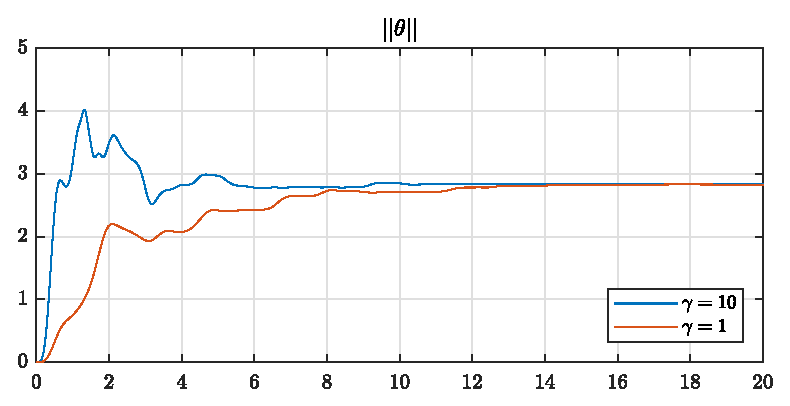
\includegraphics[width=12cm]{figs/1/modtheta/sim0gamma10gamma1.eps}
\end{figure}

\begin{figure}[H]
  \centering
  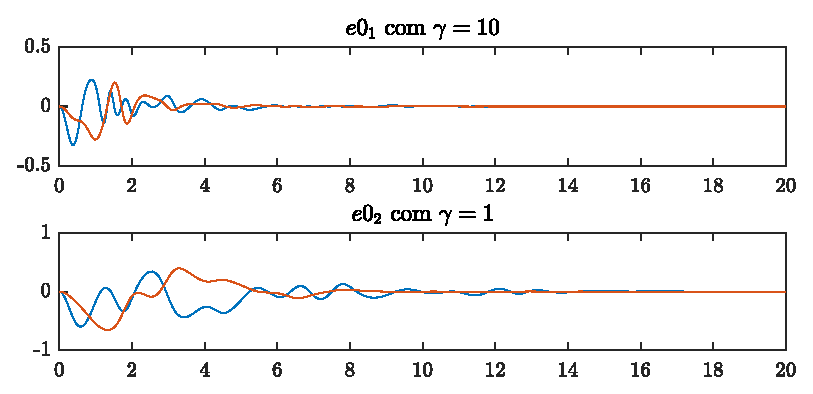
\includegraphics[width=12cm]{figs/1/e0/sim0gamma10gamma1.eps}
\end{figure}

%---------------------------------------------------------------------

\subsubsection{Simula��o \#2}

Verificamos agora o comportamento do sistema para varia��es na \textbf{condi��o inicial} $y(0)$.

\bigskip

\begin{align*}
  a_1 = a_2 &= 2 \,, &  \phi &= \frac{\pi}{3} \,, & h &= 1 \,,\\
  \theta(0) &= \mathbf{0} \,, & y(0) &= \HI{\textbf{1}} \, e \, \HI{\textbf{0}}
  \,, & \gamma &= 10\\ 
	k_m &= 2.
\end{align*}

\begin{figure}[H]
  \centering
  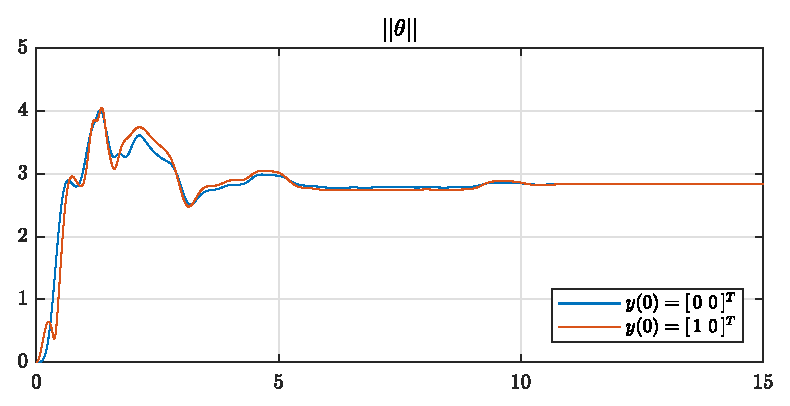
\includegraphics[width=12cm]{figs/1/modtheta/sim0y01y02.eps}
\end{figure}

\begin{figure}[H]
  \centering
  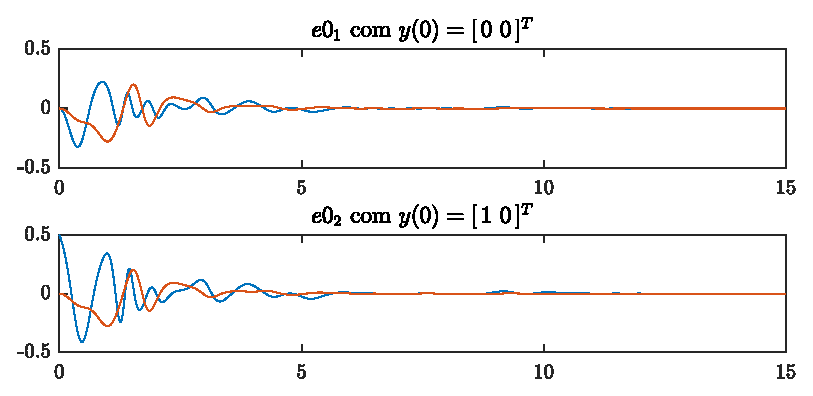
\includegraphics[width=12cm]{figs/1/e0/sim0y01y02.eps}
\end{figure}

% -----------------------------------------------------------------------------

\subsubsection{Simula��o \#3}

Verificamos o comportamento do sistema para varia��es na \textbf{fun��o de transfer�ncia da planta} $P(s)$.

\bigskip

\begin{align*}
  a_1 = a_2 &= 2 \,, &  \phi &= \HI{$\frac{\pi}{4}$} \, e
  \, \HI{$\frac{\pi}{3}$} \,, & h &= \HI{2} \, e \, \HI{1} \,,\\
  \theta(0) &= \mathbf{0} \,, & y(0) &= 0
  \,, & \gamma &= 10\\ 
	k_m &= 2.
\end{align*}

\begin{figure}[H]
  \centering
  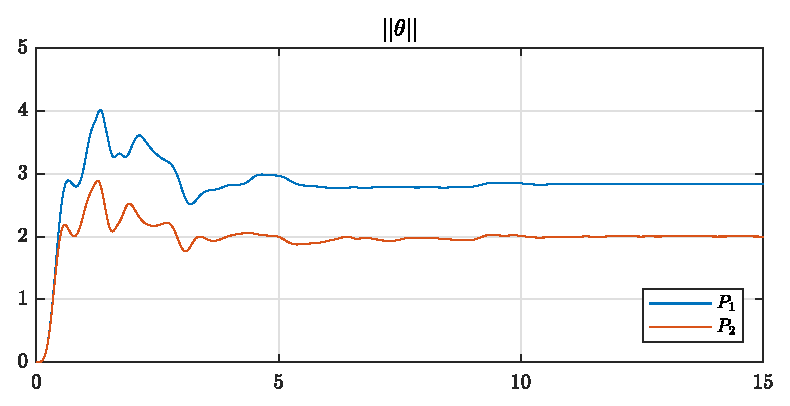
\includegraphics[width=12cm]{figs/1/modtheta/sim0P1P2.eps}
\end{figure}

\begin{figure}[H]
  \centering
  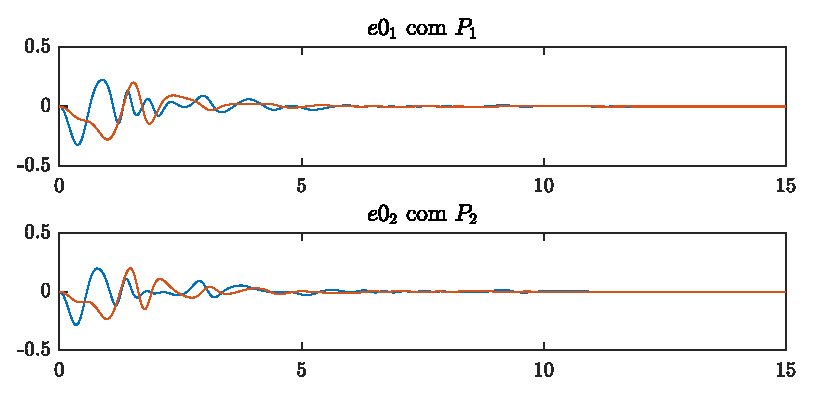
\includegraphics[width=12cm]{figs/1/e0/sim0P1P2.eps}
\end{figure}

% -----------------------------------------------------------------------------

\subsubsection{Simula��o \#4}

Verificamos o comportamento do sistema para varia��es na \textbf{fun��o de
transfer�ncia do modelo de refer�ncia} $P_m(s)$.

\bigskip

\begin{align*}
  a_1 = a_2 &= 2 \,, &  \phi &= \frac{\pi}{3} \,, & h &= 1 \,,\\
  \theta(0) &= \mathbf{0} \,, & y(0) &= \textbf{0} \,, & \gamma &= 10\\ 
	k_m &= \HI{2} \, e \, \HI{1}.
\end{align*}

\begin{figure}[H]
  \centering
  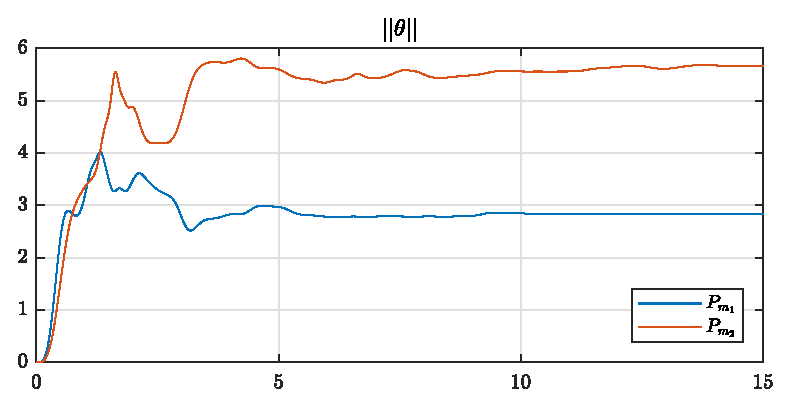
\includegraphics[width=12cm]{figs/1/modtheta/sim0Pm1Pm2.eps}
\end{figure}

\begin{figure}[H]
  \centering
  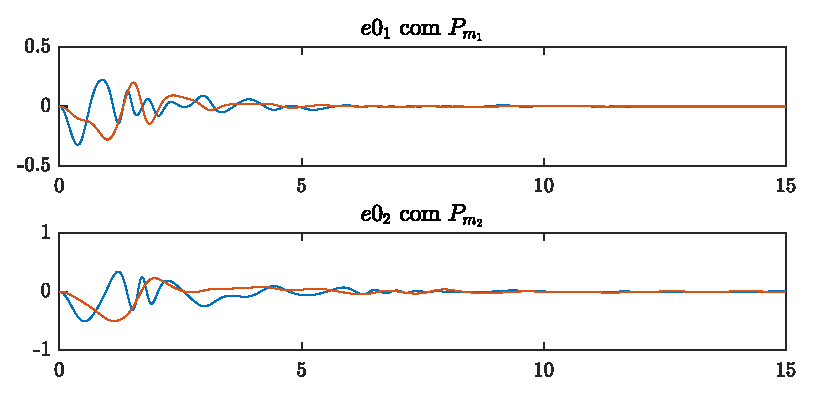
\includegraphics[width=12cm]{figs/1/e0/sim0Pm1Pm2.eps}
\end{figure}
